% Packages
\documentclass[12pt]{article}
\usepackage[margin=2.5cm]{geometry}
\usepackage{lipsum}
\usepackage{titlesec, titletoc}
\usepackage[svgnames, table]{xcolor}
\usepackage{algorithm}
\usepackage{algpseudocode}
\usepackage{mdframed}
\usepackage[T1]{fontenc}
\usepackage{amsmath,amsthm,amsfonts,amssymb,mathtools}
\usepackage[osf]{mathpazo}
\usepackage{enumitem}

% Formating setup
\footskip = 1 cm
\setlength{\parindent}{0pt}
\pdfpxdimen=1in
\parindent = 0pt
\definecolor{myBlue}{RGB}{0, 81, 255}
\titleformat{\section}[block]{\sffamily\large\bfseries}{\thesection}{.5em}{\textcolor{myBlue}
{\titlerule[1.5pt]}\\\sffamily}[\vspace*{-3mm}\textcolor{myBlue}{\titlerule[1.5pt]}]
\titleformat{\subsection}{\large\sffamily\bfseries}{\thesubsection}{0.5em}{\textcolor{Black}}
\newcounter{boxedlistcounter}
\newenvironment{pseudo}{%
  \setcounter{boxedlistcounter}{0}% <-- Add this line to reset the counter
  \mdframed[
    linecolor=black, % color of the border
    linewidth=1.5pt, % thickness of the border
    roundcorner=10pt, % radius of the corners
    innertopmargin=0.6\baselineskip, % space at the top of the box
    innerbottommargin=0.6\baselineskip, % space at the bottom of the box
  ]
  \fontsize{12pt}{14pt}\selectfont % add font size command here
  \mdseries % add font series command here
}{%
  \endmdframed%
}
\newcommand{\I}{\par\stepcounter{boxedlistcounter}\arabic{boxedlistcounter}.\hspace{5pt}}
\newcounter{boxedlistcounter2}
\newenvironment{Proof}{%
  \refstepcounter{boxedlistcounter2}%
  \mdframed[
    linecolor=black, % color of the border
    linewidth=1.5pt, % thickness of the border
    roundcorner=10pt, % radius of the corners
    innertopmargin=\baselineskip, % space at the top of the box
    innerbottommargin=\baselineskip, % space at the bottom of the box
  ]
  \fontsize{12pt}{14pt}\selectfont % add font size command here
  \mdseries % add font series command here
}{%
  \endmdframed%
}
\newcommand{\PI}{\par\textbullet\hspace{5pt}}
\setlist[itemize]{itemsep=1pt}

% Custom commands
\newcommand{\for}[1]{\textbf{for} #1 \textbf{do}}
\newcommand{\IF}[1]{\textbf{if} #1 \textbf{then}}
\newcommand{\ELSE}{\textbf{else}}
\newcommand{\return}[1]{\textbf{return} #1}
\newcommand{\assign}{ $\leftarrow$ }
\newcommand{\DEF}[2]{\textbf{def} #1(#2):}
\newcommand{\1}{\space \quad}
\newcommand{\2}{\quad \quad \quad}
\newcommand{\3}{\quad \quad \quad \quad \space}
\newcommand{\4}{\quad \quad \quad \quad \quad \quad}
\newcommand{\comment}[1]{\hfill \textit{\# #1}}

% Document start ------------------------------------------------------------------------------------
\begin{document}

% Section 1  ----------------------------------------------------------------------------------------
\section{Introduction to trees}
A tree T is made up of a set of nodes endowed with parent-child relationship with following properties:
\begin{itemize}
  \item If T is non-empty, it has a special node called the root that has no parent
  \item Every node v of T other than the root has a unique parent
  \item Following the parent relation always leads to the root (i.e., the parent-child relation does not have “cycles”)
\end{itemize}

\subsection{Terminology}
\begin{itemize}
  \item Root: node without parent.
  \item Internal node: node with at least one child.
  \item External/leaf node: node without children.
  \item Ancestors: parent, grandparent, great-grandparent, etc.
  \item Descendants: child, grandchild, great-grandchild, etc.
  \item Two nodes with the same parent are siblings. 
  \item Depth of a node: number of ancestors not including itself.
  \item Level: set of nodes with given depth.
  \item Height of a tree: maximum depth.
  \item Subtree: tree made up of some node and its descendants. 
  \item Edge: a pair of nodes (u, v) such that one is the parent of the other.
  \item Path: sequence of nodes such that consecutive nodes in the sequence have an edge
\end{itemize}
\textbf{Tree facts}
\begin{itemize}
  \item If node X is an ancestor of node Y, then Y is a descendant of X.
  \item Ancestor/descendant relations are transitive.
  \item Every node is a descendant of the root.
  \item There may be nodes where neither is an ancestor of the other.
  \item Every pair of nodes has at least one common ancestor. 
  \item The lowest common ancestor (LCA) of x and y is a node z such that z is the ancestor of x and y and no descendant of z has that property.
  \item In an ordered tree there is a prescribed order for each node’s children.
\end{itemize}

% Section 2  ----------------------------------------------------------------------------------------
\section{Traversal}
\subsection{Preorder Traversal}
To do a preorder traversal starting at a given node, we visit the node before visiting its descendants
If tree is ordered visit the child subtrees in the prescribed order. Visit does some work on the node such
as print node data, aggregate node data or modify node data. The example shows a pre\_order traversal called at
root.
\begin{pseudo}
  \I \DEF{pre\_order}{v}
  \I \1 visit(v)
  \I \1 \for{each child w of v}
  \I \2 pre\_order(w)
\end{pseudo}
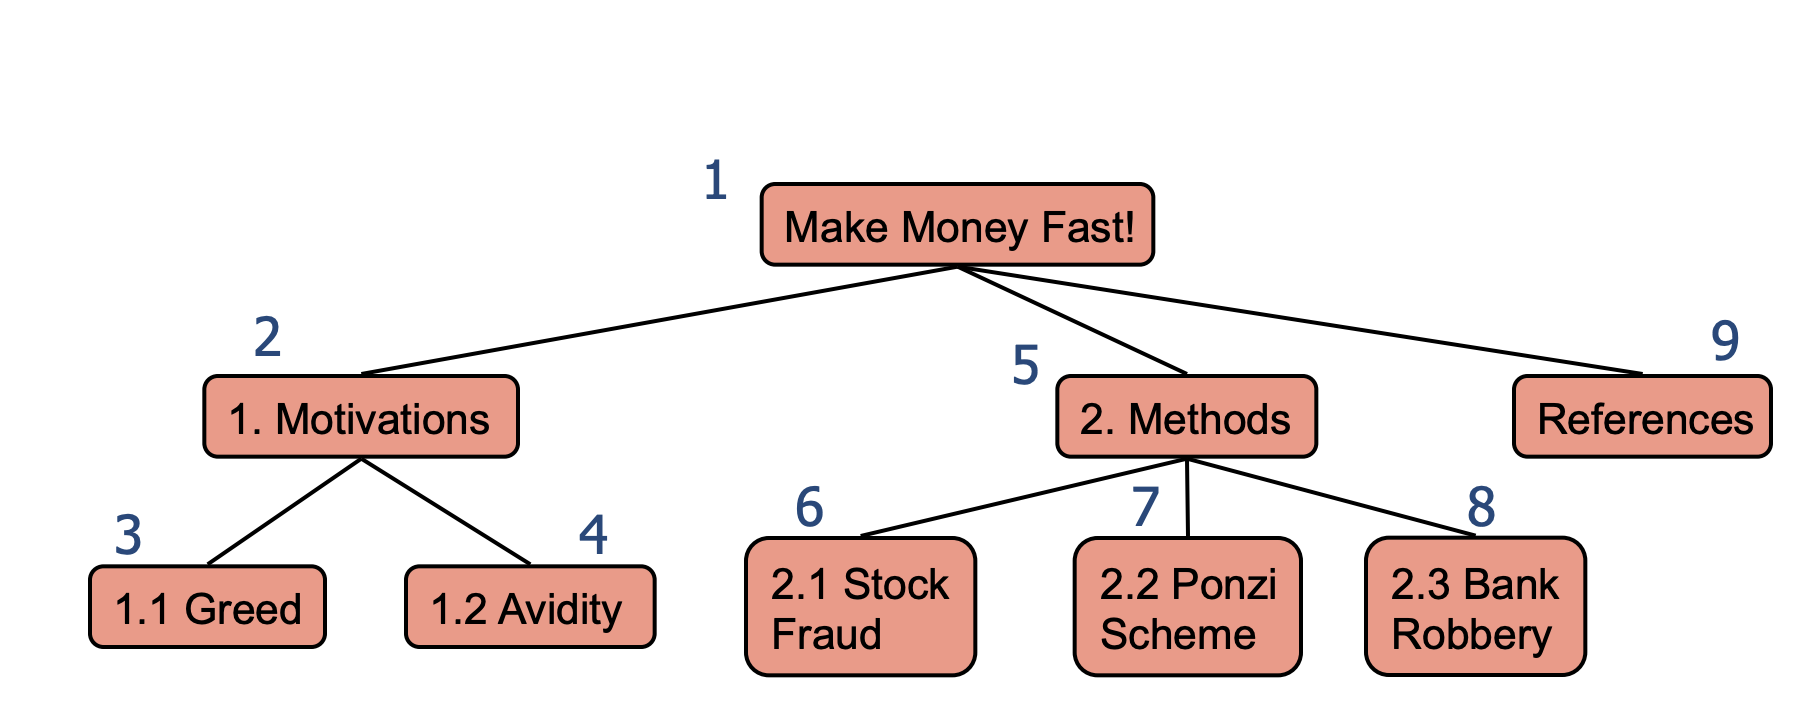
\includegraphics[width=\textwidth]{image1.png}

\subsection{Postorder Traversal}
To do a postorder traversal starting at a given node, we visit the node after its descendants
If tree is ordered visit the child subtrees in the prescribed order.
\begin{pseudo}
  \I \DEF{pre\_order}{v}
  \I \1 \for{each child w of v}
  \I \2 pre\_order(w)
  \I \1 visit(v)
\end{pseudo}
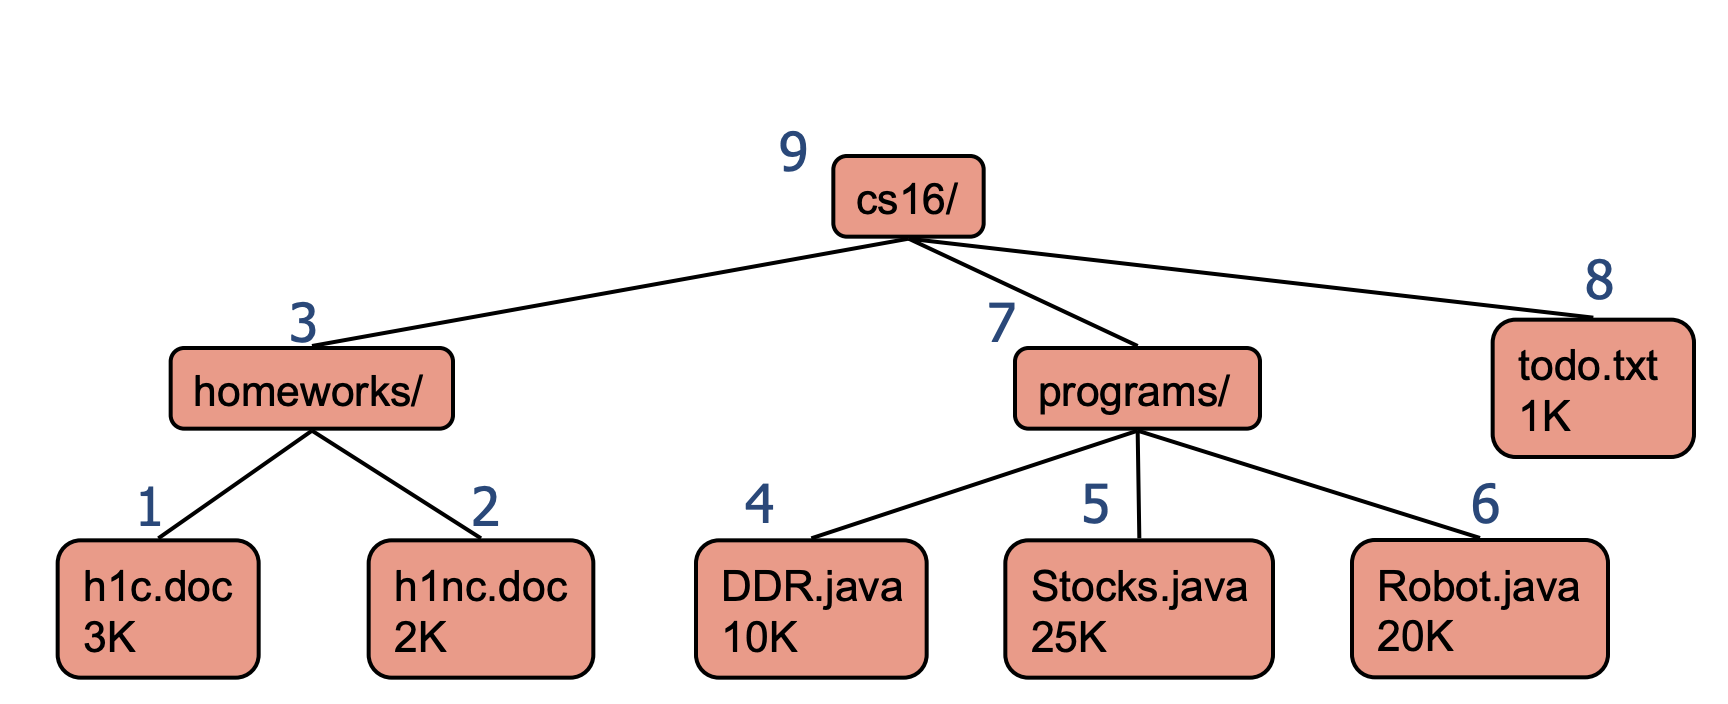
\includegraphics[width=\textwidth]{image2.png}

% Section 3  ----------------------------------------------------------------------------------------
\section{Binary Trees}
A binary tree is an ordered tree with the following properties: Each internal node has at most two children.
Each child node is labeled as a left child or a right child. Child ordering is left followed by right.
The right/left subtree is the subtree root at the right/left child. We say the tree is proper if every
internal node has two children.
\begin{pseudo}
  \I \DEF{is\_external}{v} \comment{Tests if v is a leaf}
  \I \1 \return{v.left = null and v.right = null}
\end{pseudo}

\subsection{Inorder Traversal}
To do an inorder traversal starting at a given node, the node is visited after its left subtree 
but before its right subtree.

\begin{minipage}[l]{0.6\textwidth}
  \begin{pseudo}
    \I \DEF{in\_order}{v}
    \I \1 \IF{v.left != null}
    \I \2 in\_order(v.left)
    \I \1 visit(v)
    \I \1 \IF{v.right != null}
    \I \2 in\_order(v.right)
  \end{pseudo}
\end{minipage}
\begin{minipage}[r]{0.39\textwidth}
  \raggedleft
  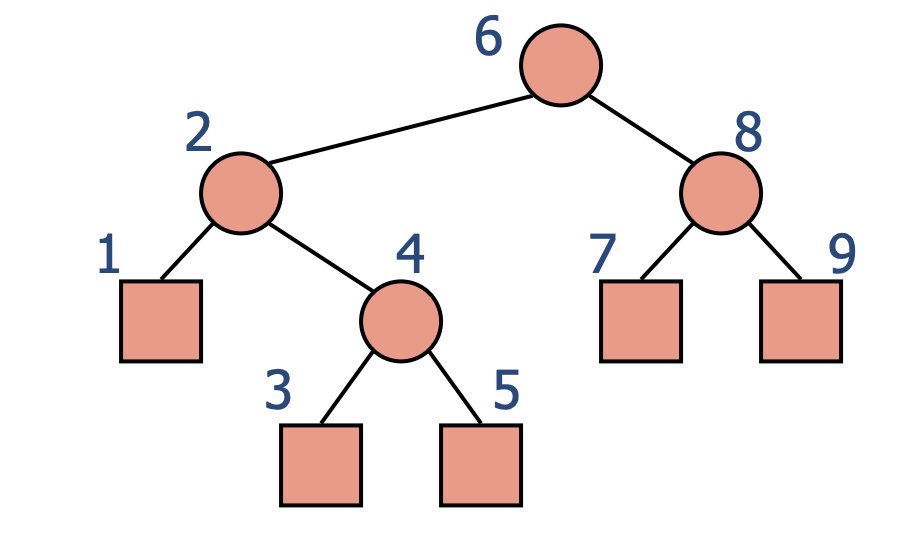
\includegraphics[width=\textwidth]{image3.png}
\end{minipage}

% Section 3  ----------------------------------------------------------------------------------------
\section{Euler Tour Traversal \& Some code}
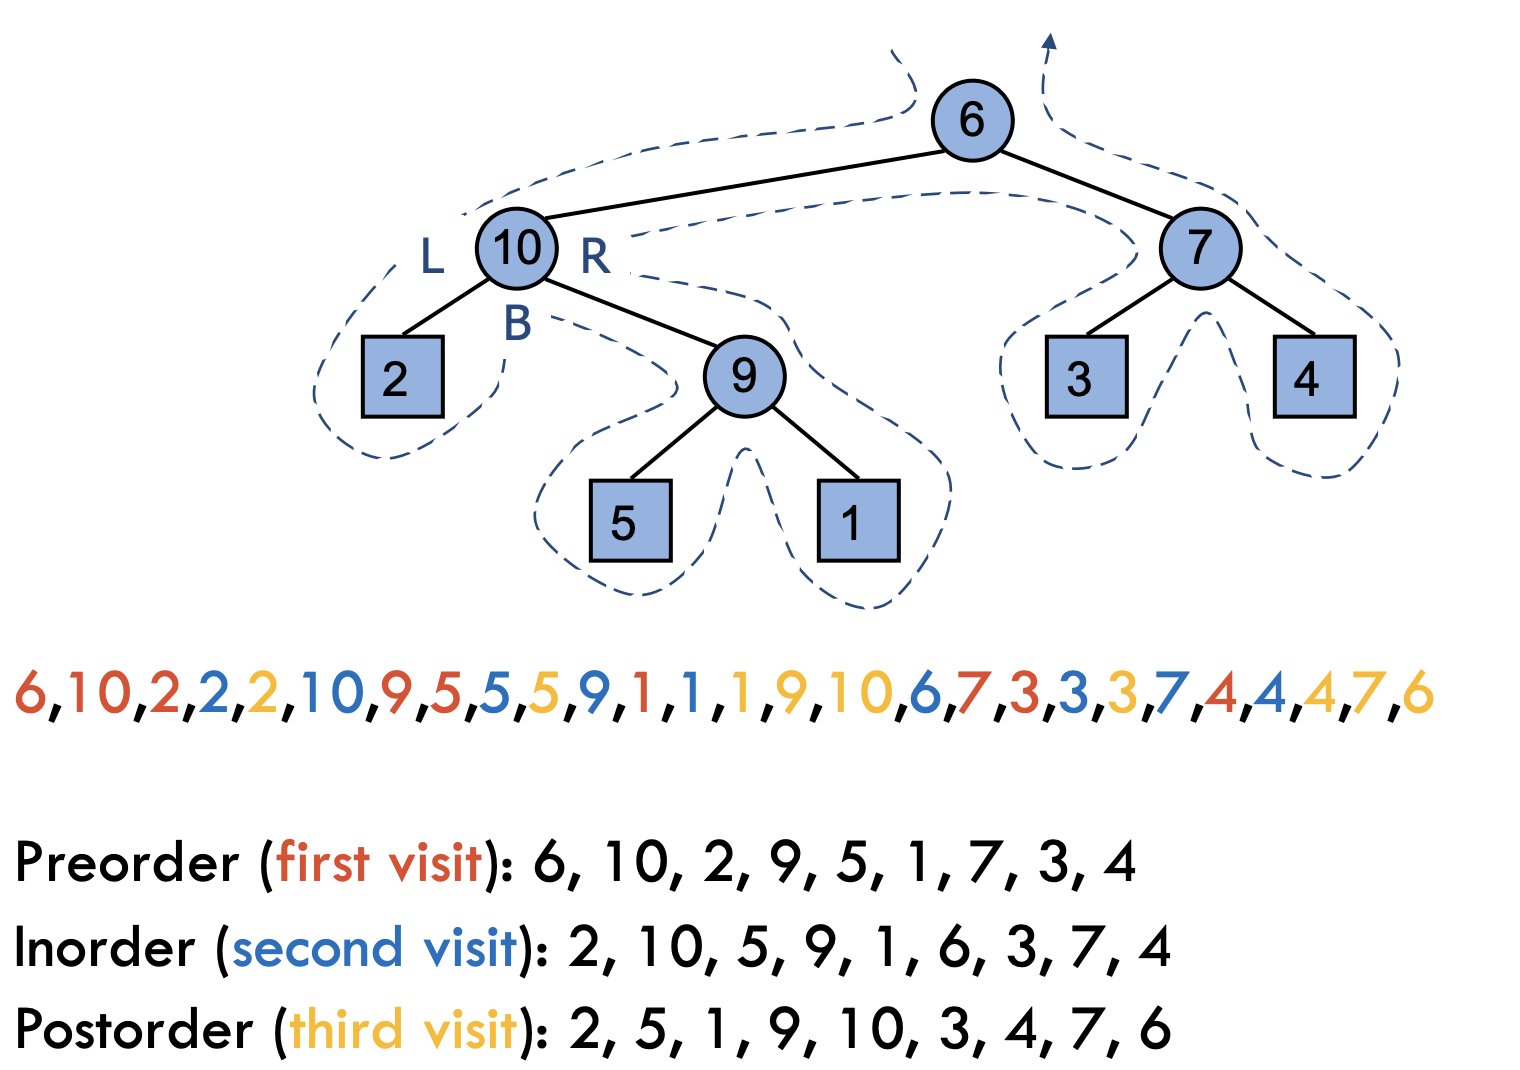
\includegraphics[width=0.90\textwidth]{image4.png}
\vspace{20pt}
\begin{pseudo}
  \I \DEF{height}{v} \comment{compute height of subtree at v}
  \I \1 \IF{v.parent = null} \comment{root’s depth is 0}
  \I \2 \return{$0$}
  \I \1 \ELSE
  \I \2 \return{depth(v.parent) + 1}
\end{pseudo}
\begin{pseudo}
  \I \DEF{depth}{v} \comment{compute height of subtree at v}
  \I \1 \IF{v.isExternal()} \comment{a leave’s height is $0$}
  \I \2 \return{$0$}
  \I \1 \ELSE{}
  \I \2 h \assign $0$
  \I \2 \for{each child w of v}
  \I \3 h \assign max(h, height(w))
  \I \2 \return{h + 1}
\end{pseudo}












\end{document}


